% !TeX root = ../main.tex
% Add the above to each chapter to make compiling the PDF easier in some editors.

\chapter{Design}\label{chapter:design}

The previous chapter introduced the core design of LAIK and the IPC mechanisms used in our implementation.
The following chapter explains the top level architecture of our shared memory backend. 
We design two versions of our shared memory backend: a standalone version able  to run on a single node and an integragted version which supports another backend with efficient shared memory based inter node communication.
We first explain how the backend initializes itself and transports data over shared memory.
We then move on to explain how the standalone version was changed to be able to function as a secondary backend assisting another Backend with a different communication library.

\section{Initialization} \label{section:initialization}

To be able to transport data across our processes, the processes first have to get aware of their peers and establish adresses to be able to adress another. 
During initialization, the processes establish the required means of communication as well as a master process.
After initialization, every process needs to be aware of its own adress and the size of the group.

\begin{figure}[h]
	\centering
	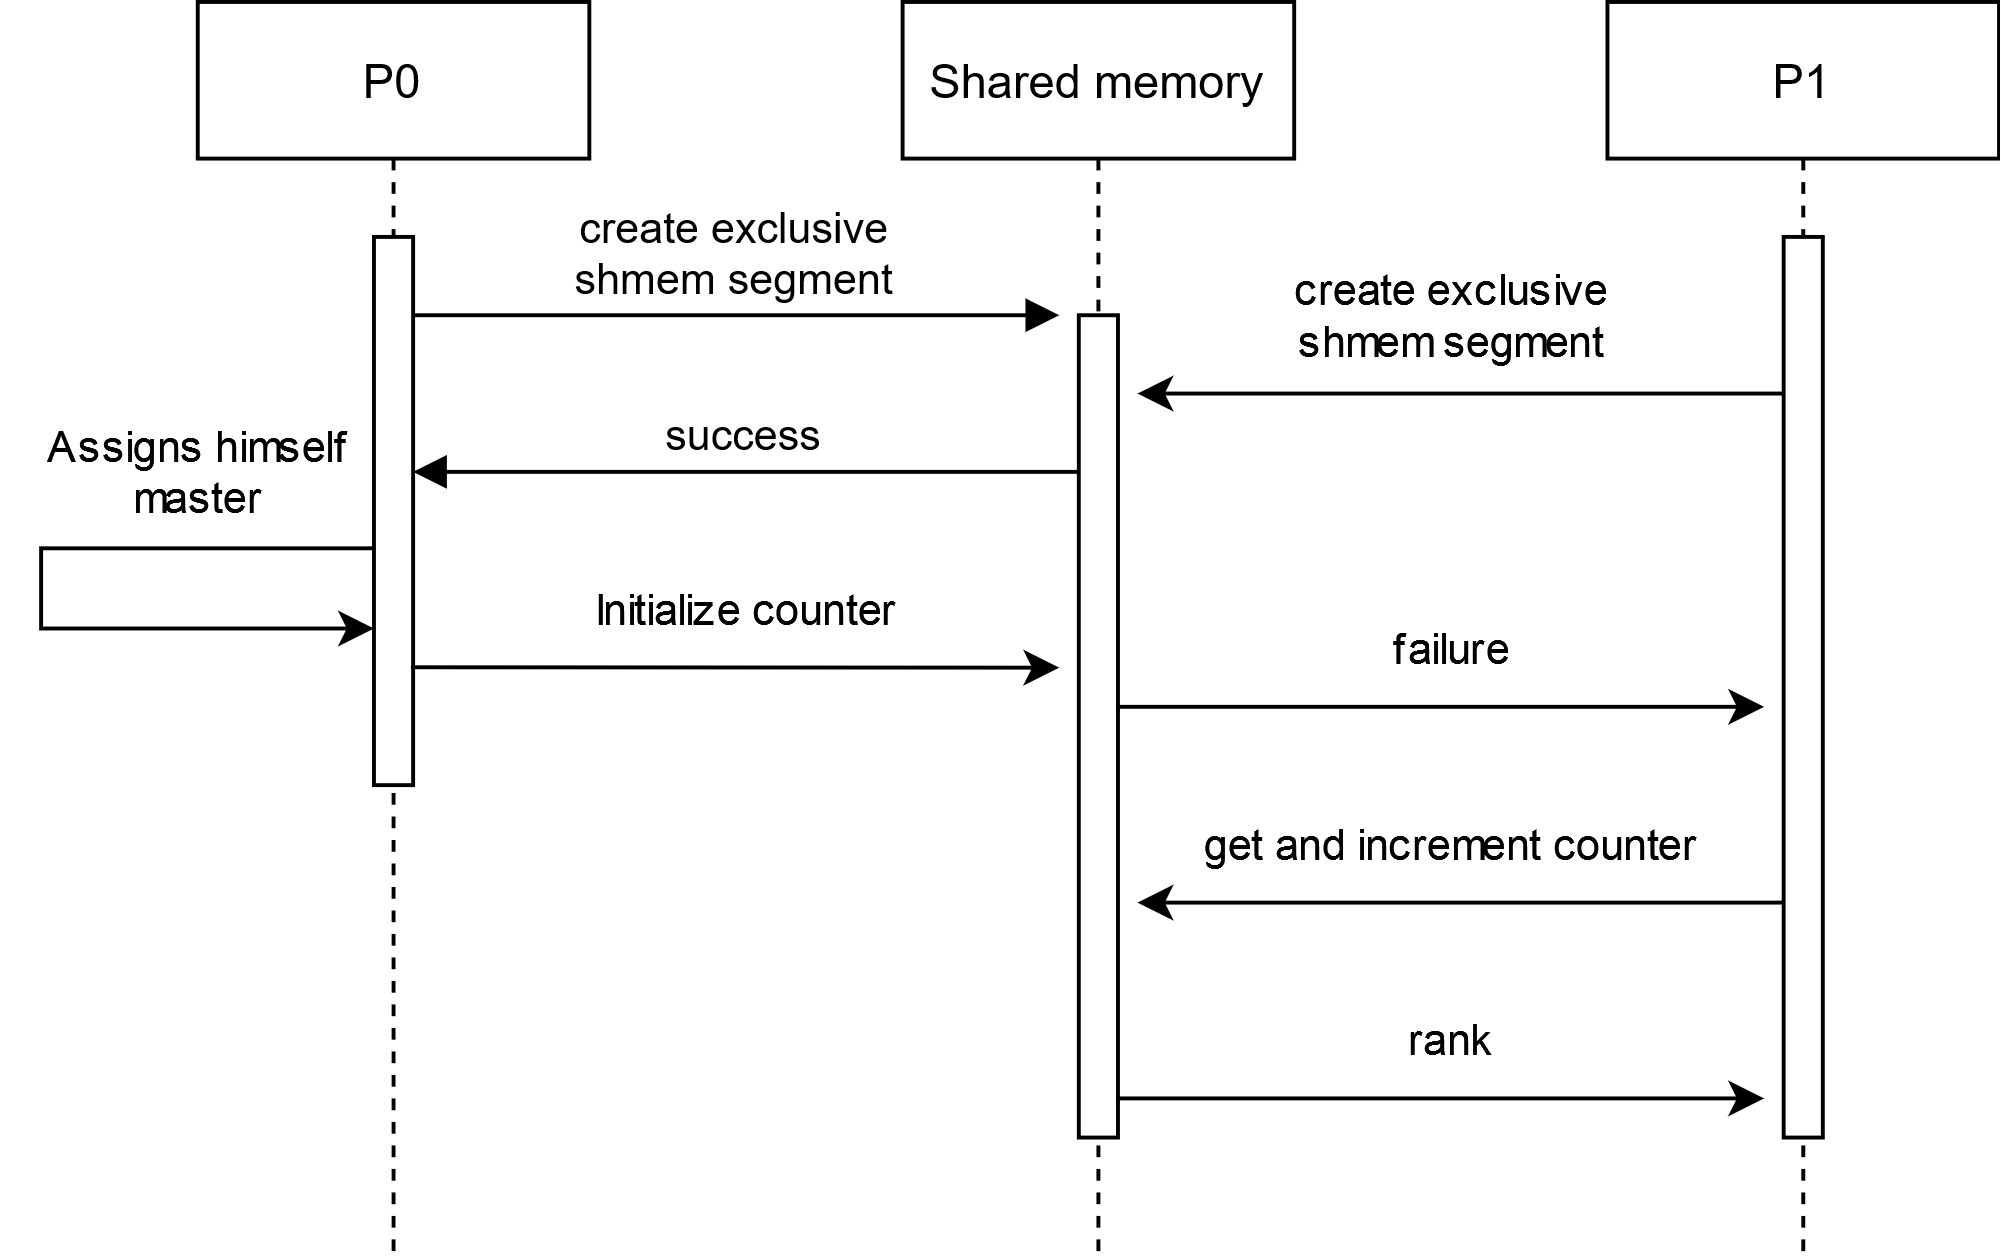
\includegraphics[width=0.75\columnwidth]{figures/initialization.png}
	\caption{Exemplary process of an initialization with two processes}
	\label{fig:initialization}
\end{figure}

To start the initialization, the processes first need to establish a preliminary means of communication on which they can assign their addresses.
Those addresses will be called ranks in the following.
To start initialization, all processes will try to create the same exclusive shared memory segment.
That way only one process can succeed in creating this segment.
This process assigns himself the rank $0$ which means he will be the master of the group.
He will also initialize a counter in the created shared memory segment which will be used to assign the processes their ranks.
All other processes are going to fail at creating the exclusive shared memory segment, which means they will be client processes.
Those processes will then open and access the segment to increment the counter and assign themselves the new counter value as their rank.
For example in \autoref{fig:initialization} the first process P0 succeeds in creating the segment, assigns himself master and initializes the counter.
The second process P1 then fails to create the segment because the first one already did.
It then increments the counters value and assigns himself the current value as rank.

\section{Data Transport}\label{section:design_data_transport}

The data transport is the core of our backend, without it no data migration would be possible.
To perform the data transport over shared memory we implemented two versions: a 2 copy and a 1 copy version.
A 2 copy version is needed because LAIK allows applications to directly provide memory.
Directly provided memory is memory that is allocated by the application and not by LAIKs allocator.
If such a memory space sends data, the receiving party can not directly copy out of the segment because it is not a shared one.
In that case a 2 copy version the only viable option.
However, the 2 copy version only serves as a fallback when a 1 copy transport is not possible.

\subsection{2 Copy Transport}

In order to accommodate the transport of data from directly provided memory we implemented a 2 copy data transport. 
This means that any data sent with this method is copied two times during transport as can be seen in \autoref{fig:2copy}. 
The sending process creates a new shared memory segment and attaches to it. 
The process then copies the relevant segment to the shared segment. 
The receiving process opens the shared segment and copies the data to his own segment.
After that the shared memory segment is destroyed.

\begin{figure}[h]
	\centering
	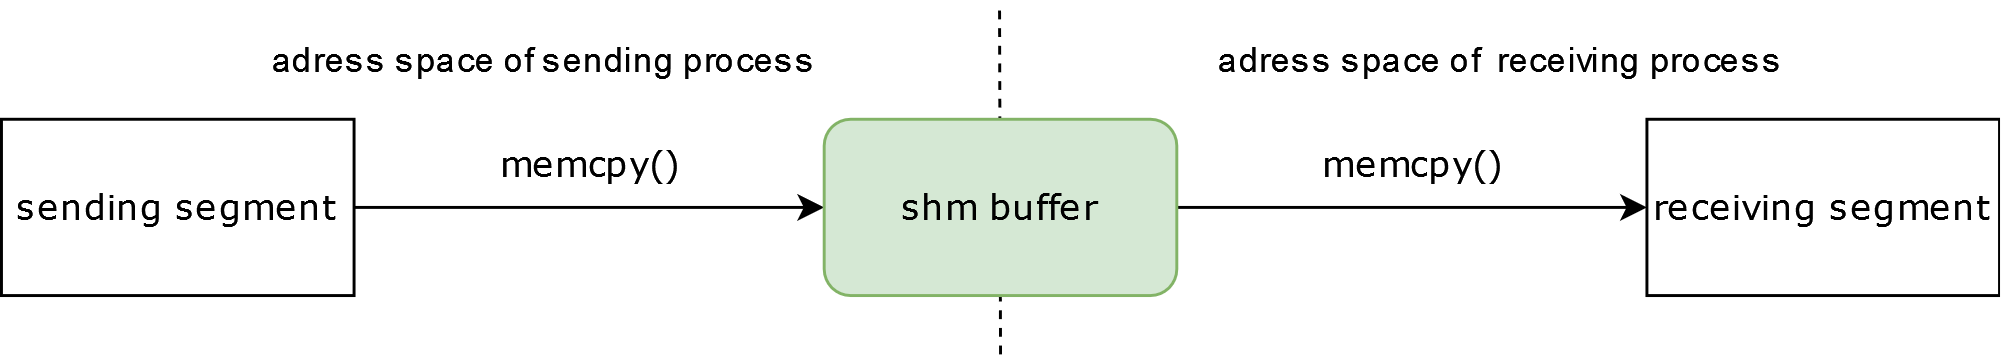
\includegraphics[width=1.00\columnwidth]{figures/2copy.png}
	\caption{Schematic of the 2 copy transport}
	\label{fig:2copy}
\end{figure}

\subsection{1 Copy Transport}

As the copying of the segment is the most resource intense operation of a data transmission operation, it makes sense to copy only once.
We therefore design a 1 copy version of our data transport over shared memory.
In contrast to the 2 copy version, both segments are shared segments which allows the sending and receiving processes to copy directly from one to the other.
For this the sending process marks the segment as ready so that the receiving process can copy it directly into his own memory. 
The receiving process waits until the segment he wants to copy from is marked as ready and then copies it into his own segment.
As we can be seen in \autoref{fig:1copy} we can save one \code{memcpy()} call this way, which should increase the throughput of our backend.

\begin{figure}[h]
	\centering
	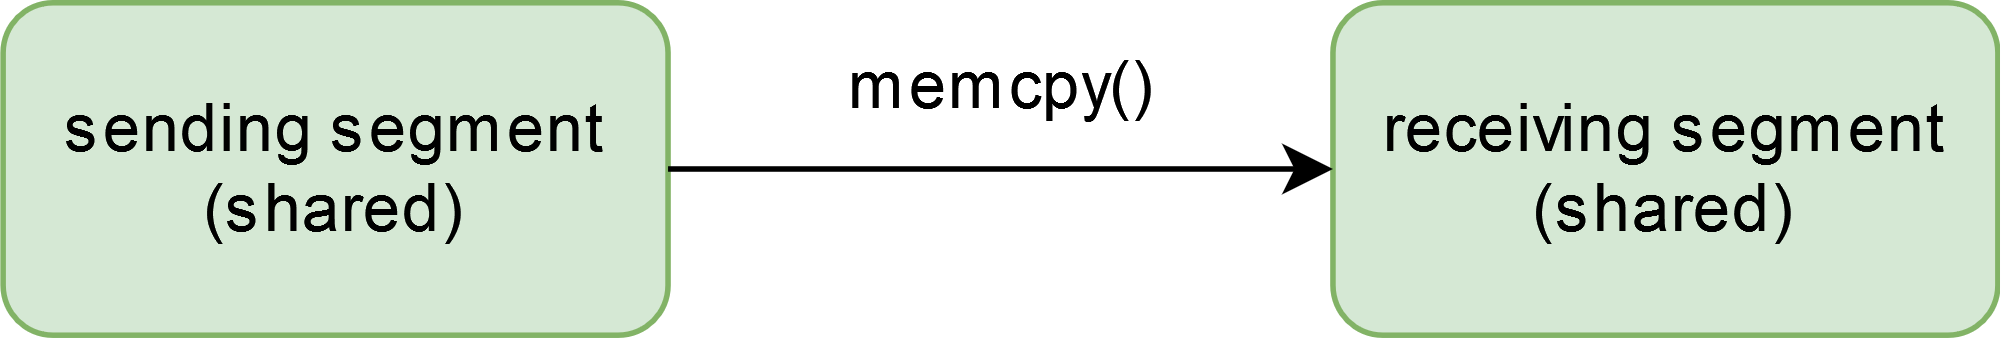
\includegraphics[width=0.66\columnwidth]{figures/1copy.png}
	\caption{Schematic of the 1 copy transport}
	\label{fig:1copy}
\end{figure}


\section{Standalone Version}

The standalone version we developed only uses shared memory to fulfil its tasks and can therefore only run on a single node.
This version is not able to run across nodes as the shared memory of one node is not accessible from another node.
The standalone version implements all necessary backend functions and is therefore able to run on its own.
The methods the standalone backend implements from the backend interface are similar to those of the MPI backend. 
Only the data transport was replaced by our shared memory based transport.
This backend works like a normal backend, it prepares, executes and cleans up his action sequences by itself.
The backend can therefore be used like any other backend as long as the application runs on a single node.

\section{Secondary Backend Version}

The secondary backend version was created to be able to run on multiple nodes.
In the example in \autoref{fig:clusters} we have 2 clusters with 2 processes each.
The 2 pairs of processes on the same node would be able to communicate with each other over shared memory but not with the other pair, as it is not possible to use shared memory for inter node communication.
The shared memory backend therefore needs to be combined with another communication backend to be able to deploy an application on multiple nodes.
The shared memory backend should therefore only support the other communication backend with providing efficient intra node communication.
The backend that uses the shared memory backend will be called primary backend and the shared memory backend will be called secondary backend.
The secondary backends tasks get reduced to replacing normal actions with shared memory actions where possible and executing those shared memory actions.
The primary backend will function as a normal backend which delegates its actions to shared memory where possible.
The secondary backend should be easy to integrate into new backends as most backends should profit from its support. 

\begin{figure}[h]
	\centering
	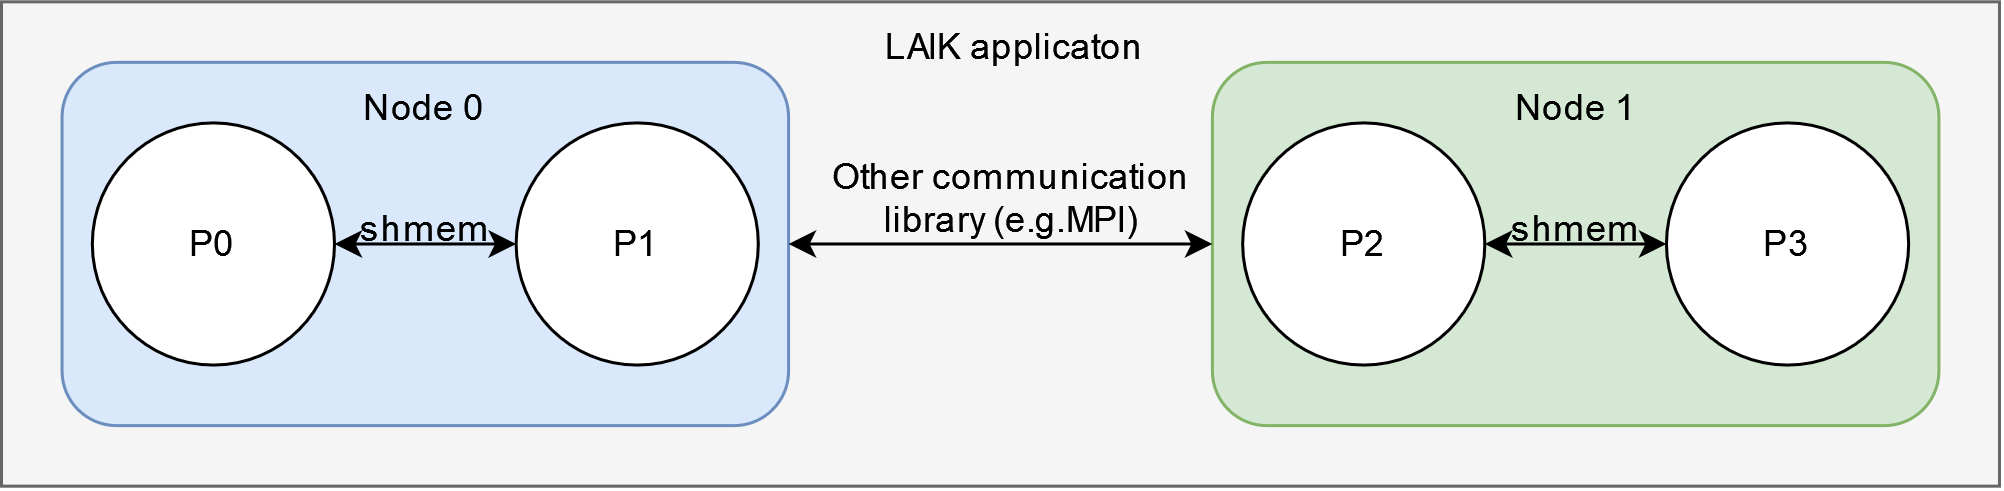
\includegraphics[width=0.90\columnwidth]{figures/clusters.png}
	\caption{Exemplary deployment of an application with 4 processes on 2 nodes}
	\label{fig:clusters}
\end{figure}

\subsection{Integration into Other Backends}

The secondary backend version is not able to run standalone, it therefore needs to be integrated into another backend to run.
As most backends should profit from the support of the shared memory backend, the backend should be able to be easily integrated into any other LAIK backend.
A backend should therefore need as few modifications as possible to integrate the secondary version as its secondary backend. 
The primary backend should only have to call one initialization method to initialize the shared memory backend.
After that the primary backend should be able to optimize and execute all its action sequences with the help of the secondary backend.
After an action sequence is optimised with shared memory all actions between processes on the same node should be replaced with shared memory based actions.
During execution of an action sequence the primary backend will then execute all actions which involve processes on different nodes.
Those actions will then be executed with the primary's communication library.
All other actions will be delegated to the secondary backend to be executed there.

\subsection{Initialization of multiple Shared Memory Clusters}\label{section:init_multiple_clusters}

As the secondary backend versions purpose is to use shared memory where possible when deploying an application across nodes, we have to manage different shared memory clusters.
A shared memory cluster are all processes of an application which can communicate with each other via shared memory.
In the example seen in \autoref{fig:initialization} we would have 2 clusters with 2 processes each (\{0, 1\}, \{2, 3\}).
If we would now initialize all four processes with the method presented \autoref{section:initialization} we would get 2 clusters, but the two clusters would not be aware of each other.
The secondary backend version will therefore use the primary backends communication library to get aware of other clusters.
After initialization each process should be aware of all other processes and their cluster affiliation.

\subsection{Action Substitution}

To use the secondary backend, the primary backend must substitute its generic actions with shared memory based actions during preparation.
The secondary backend must provide an optimization pass for that purpose which the primary backend can use during preparation of an action sequence.
This optimization pass should iterate over every action and check whether the involved processes are on the same node.
If so, the action can and should be replaced by its corresponding shared memory action.
The returned action sequence can then be further optimized by the primary backend to change the remaining generic actions.